3.

Создадим новый ориентированный граф $G'$ на основе данного $G$. Каждой вершине $u \in G$, кроме начальной и конечной поставим в соответствие вершины $u_{in} \in G'$ и $u_{out} \in G'$, и соединим их (ориентированными) ребрами $(u_{in}, u_{out})$. Теперь проводим ребра: если $(u, v) \in G$, то проводим $(u_{out}, v_{in}) \in G'$ и $(v_{out}, u_{in}) \in G'$. В конце проводим ребра от начальной вершины: если $(s, u) \in G$, то проводим $(s', u_{in}) \in G'$. Аналогично для конечной вершины, но в обратную сторону. Веса всех ребер делаем равными $1$. Теперь пускаем максимальный поток из $s'$ в $t'$. Это и будет ответом.

Если искать минимальный поток с помощью алгоритма Форда-Фалкерсона, то получим $O(\mathit{ans}(n + 2m)) = O(\mathit{ans}(n + m))$. Если с помощью Эдмонса-Карпа, то $O\left(2n \cdot (n + 2m)^2) = O(n^3 + n^2 m + nm^2\right)$. Если с помощью Диница, то число итераций равно $\sqrt{P} = \sqrt{1 \cdot 2n}$, т.к. потенциал каждой вершины равен $1$, а всего вершин $2n$ (с точностью до константы), и асимптотика равна $O\left(\sqrt{2n} \cdot (2n \cdot (n + 2m))\right) = O\left(n^{\frac{5}{2}} + n^{\frac{3}{2}} m\right)$.

\begin{center}
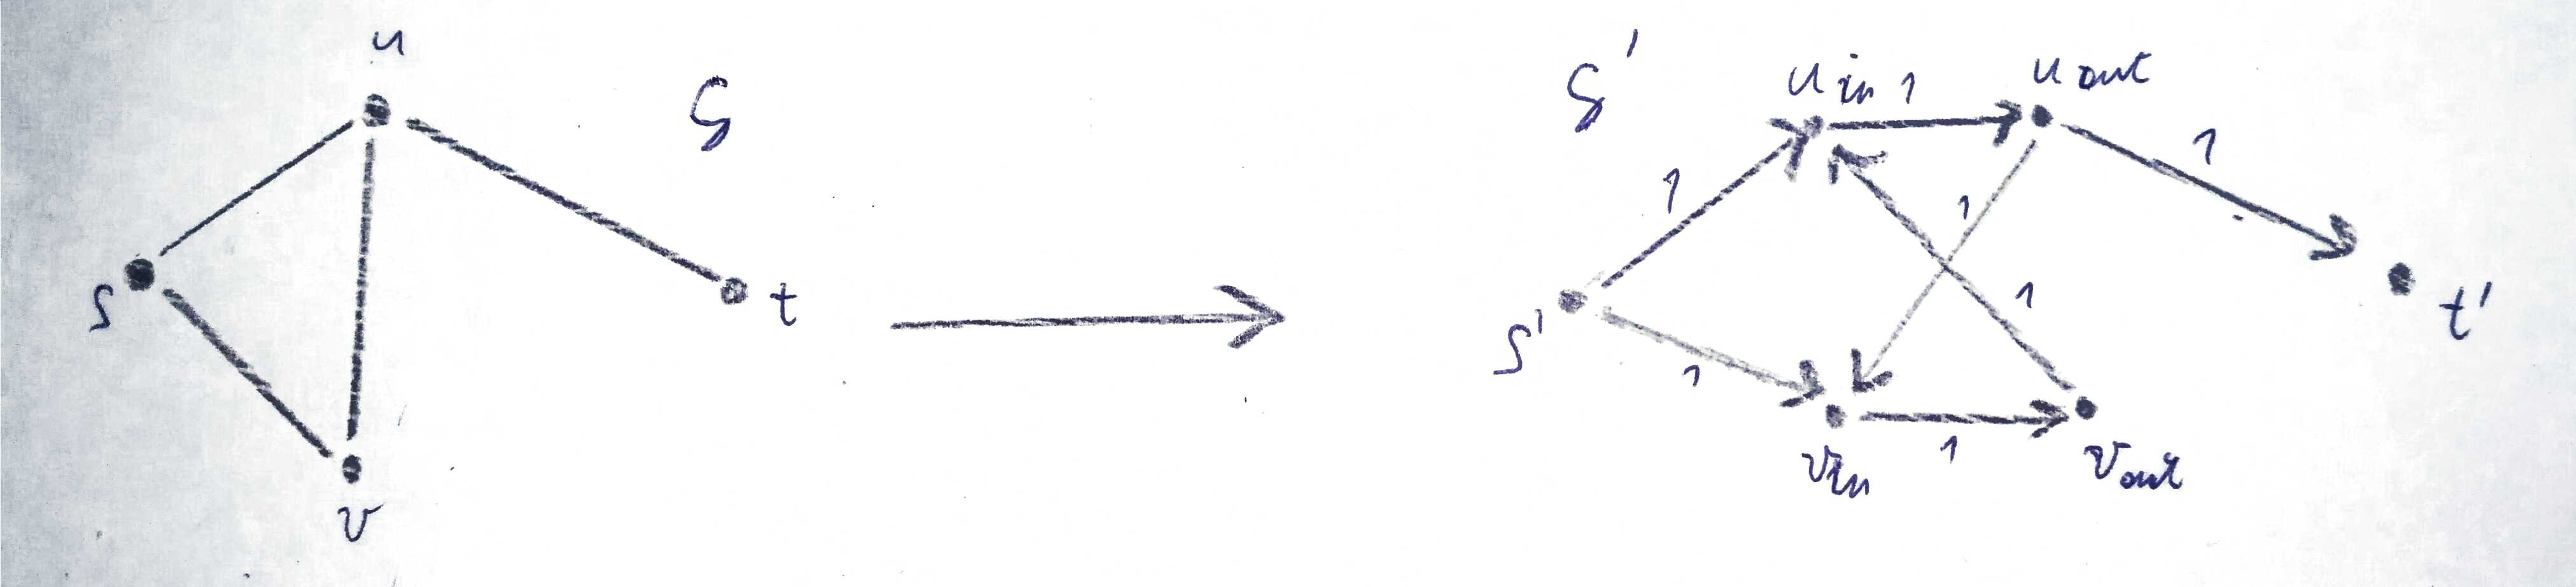
\includegraphics[width = 5in]{solution-3.jpg}
\end{center}